\documentclass[12pt, a4paper]{article}

\usepackage{graphicx}


\title{Notulensi Pertemuan}
\author{BMKG 2}
\date{24 July 2022}

\begin{document}
\maketitle

\begin{tabbing}
\textbf{Hari/Tanggal}\quad\= Minggu, 24 July 2022 \\
\textbf{Waktu} \>19.30 - 21.30 \\
\textbf{Tempat}\> Zoom Meeting
\end{tabbing}

Agenda pertemuan hari ini adalah:
\begin{enumerate}
\item gladi resik presentasi
\item pembuatan video presentasi
\item diskusi mengenai \emph{Github}
\end{enumerate}

\bigskip 
Pertemuan kali ini adalah pertemuan terakhir sebelum batas pengumpulan \emph{demo day}, agenda hari ini adalah kami ingin membuat video presentasi yang akan dikumpulkan tanggal \textbf{27 Juli 2022}. Sebelum membuat video presentasi kami memeriksa kembali konten yang kemarin sudah dibuat lalu melakukan gladi resik. Setelah semua siap, kami mulai merekam untuk keperluan video presentasi seperti urutan yang sudah ditentukan pada pertemuan sebelumnya.

\medskip
Video presentasi kami ternyata lebih dari 10 menit sehingga diperlukan adanya proses \emph{editing} lebih lanjut yang akan dikerjakan oleh Krisna. Agenda selanjutnya adalah membahas terkait penggunaan Github yang disyaratkan oleh panita. Kami membahas tentang bagaimana cara untuk mengupload data yang sudah kami kerjakan kedalam \emph{repository} Github kelompok yang sudah dibuat.

\medskip
Hal yang perlu diperhatikan selanjutnya adalah review konten video yang telah melewati proses \emph{editing} dan pembuatan laporan akhir.


\bigskip
\section*{Dokumentasi}

\begin{figure}[h]
    \centering
    \includegraphics[width=\textwidth]{pert-4.5}
    \caption{Pertemuan Ke-4}
\end{figure}

\begin{figure}[h]
    \centering
    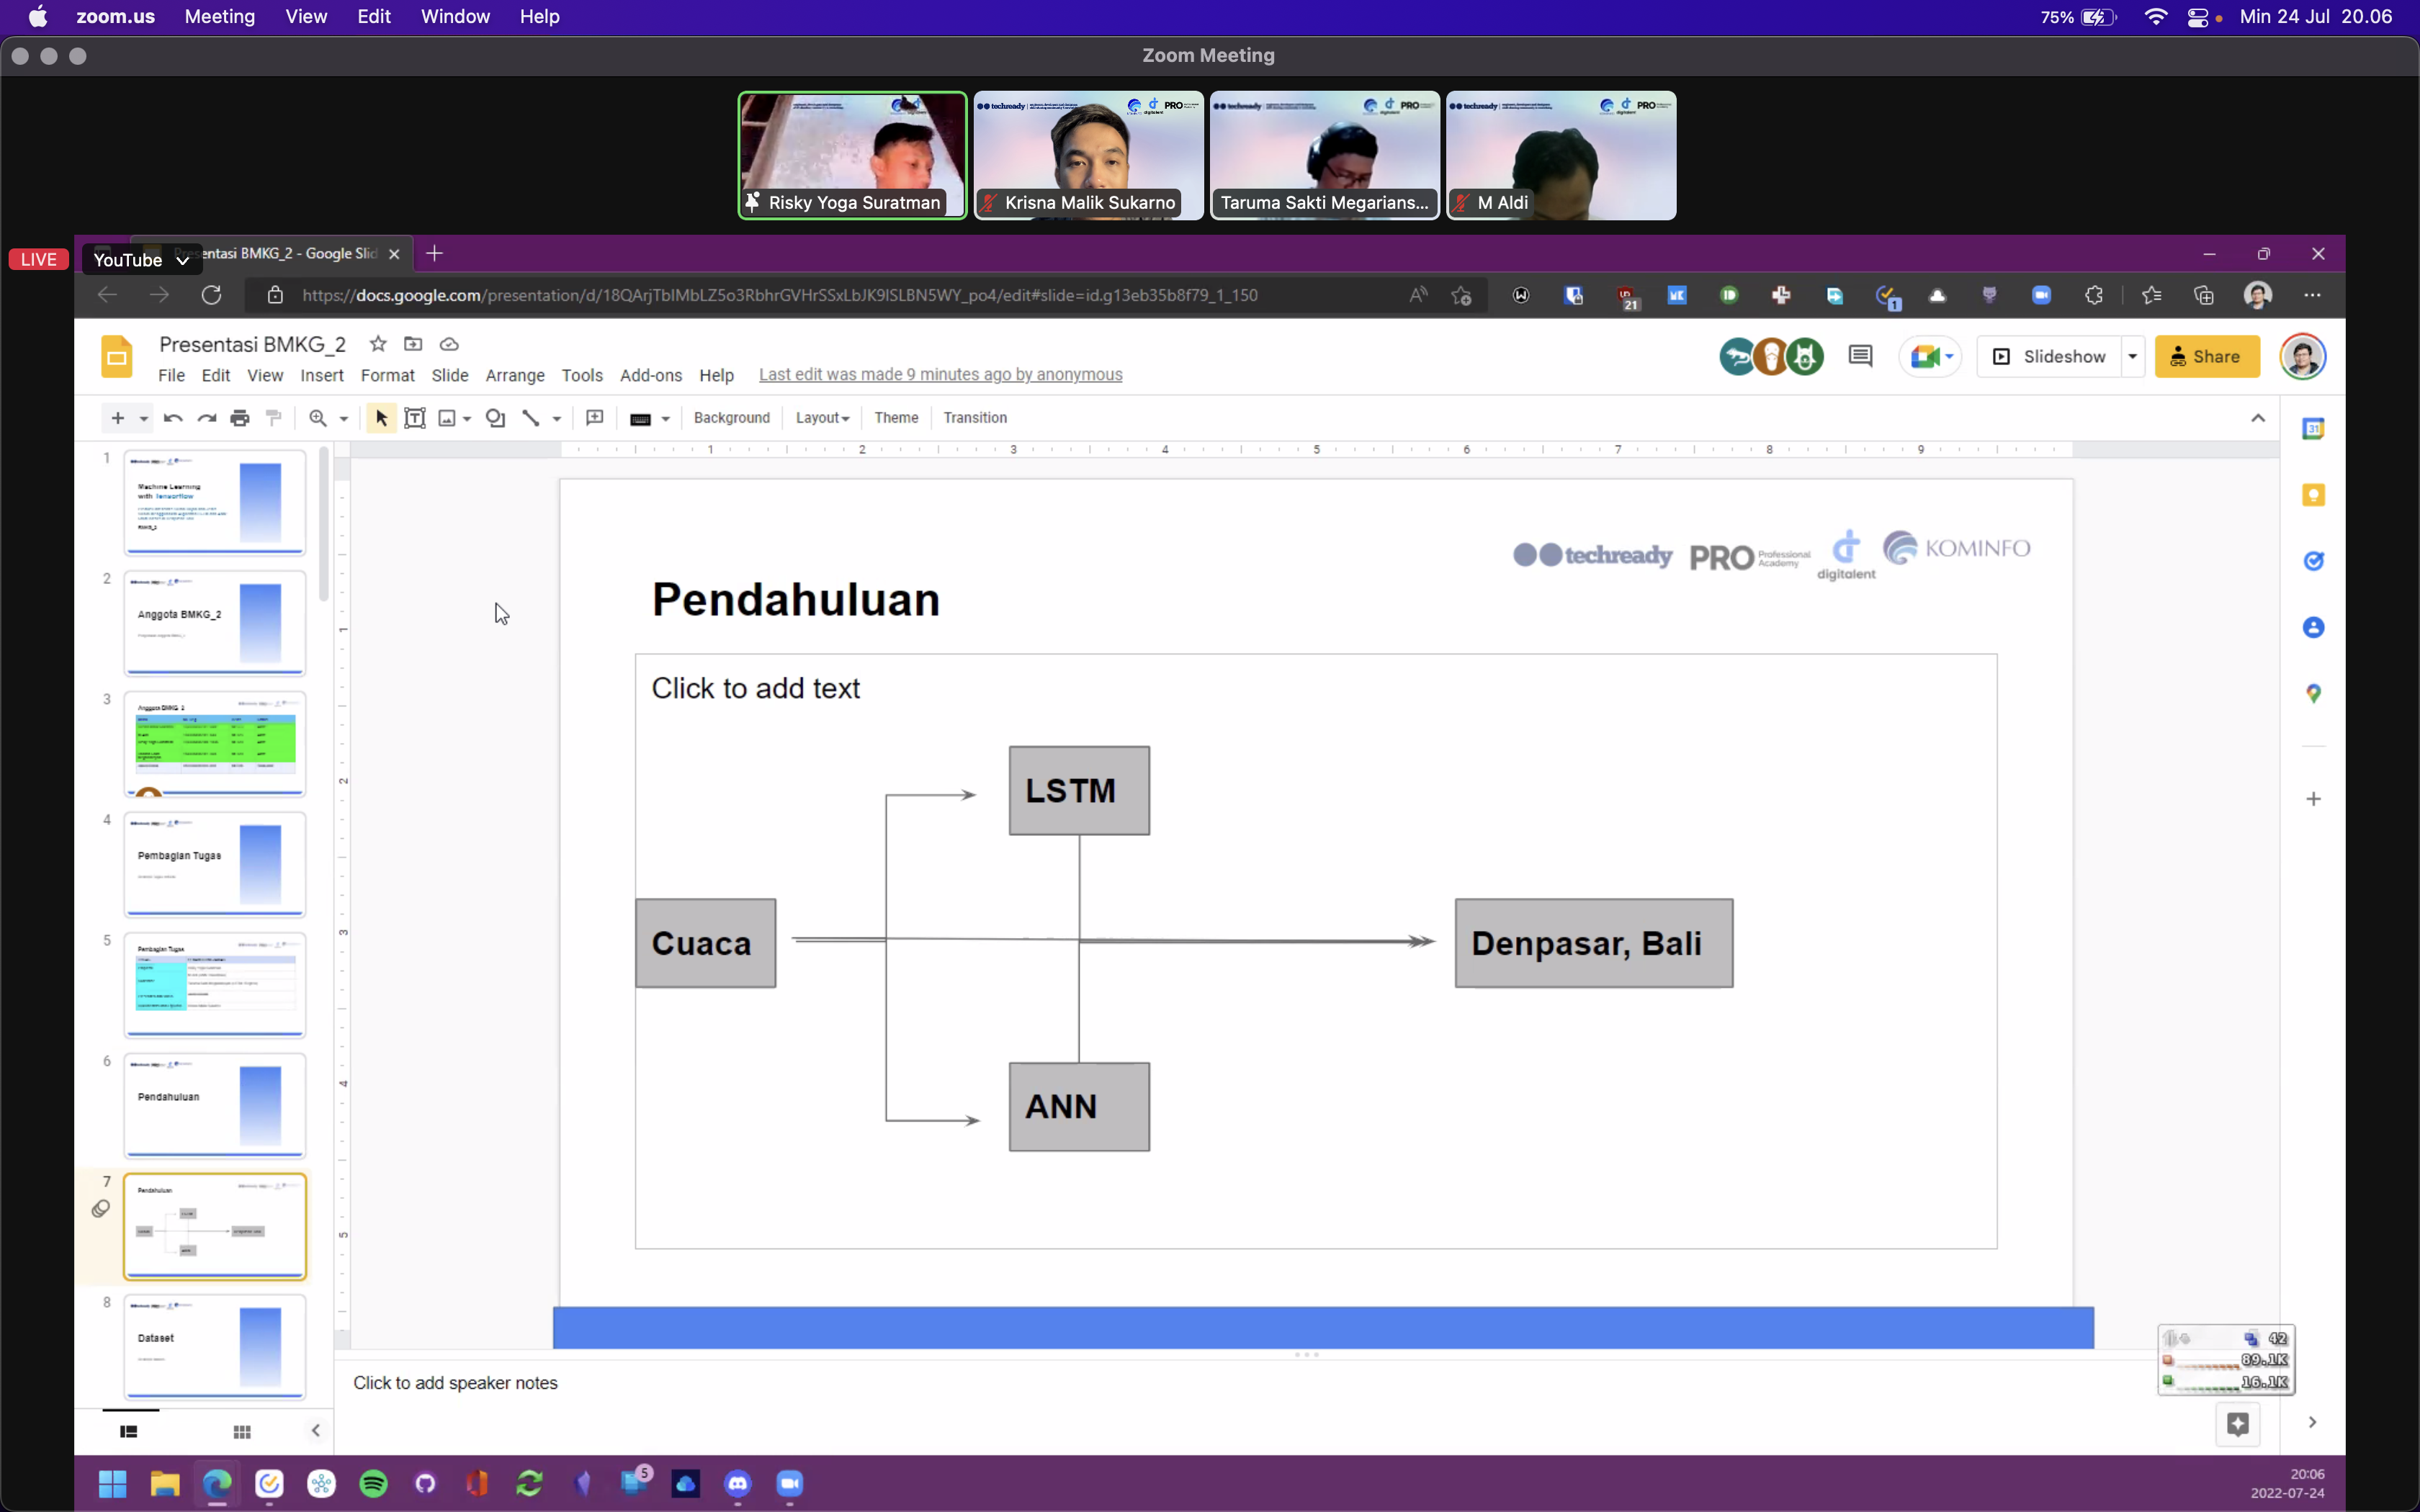
\includegraphics[width=\textwidth]{pert-4.2}
    \caption{Diskusi terkait presentasi}
\end{figure}

\begin{figure}[h]
    \centering
    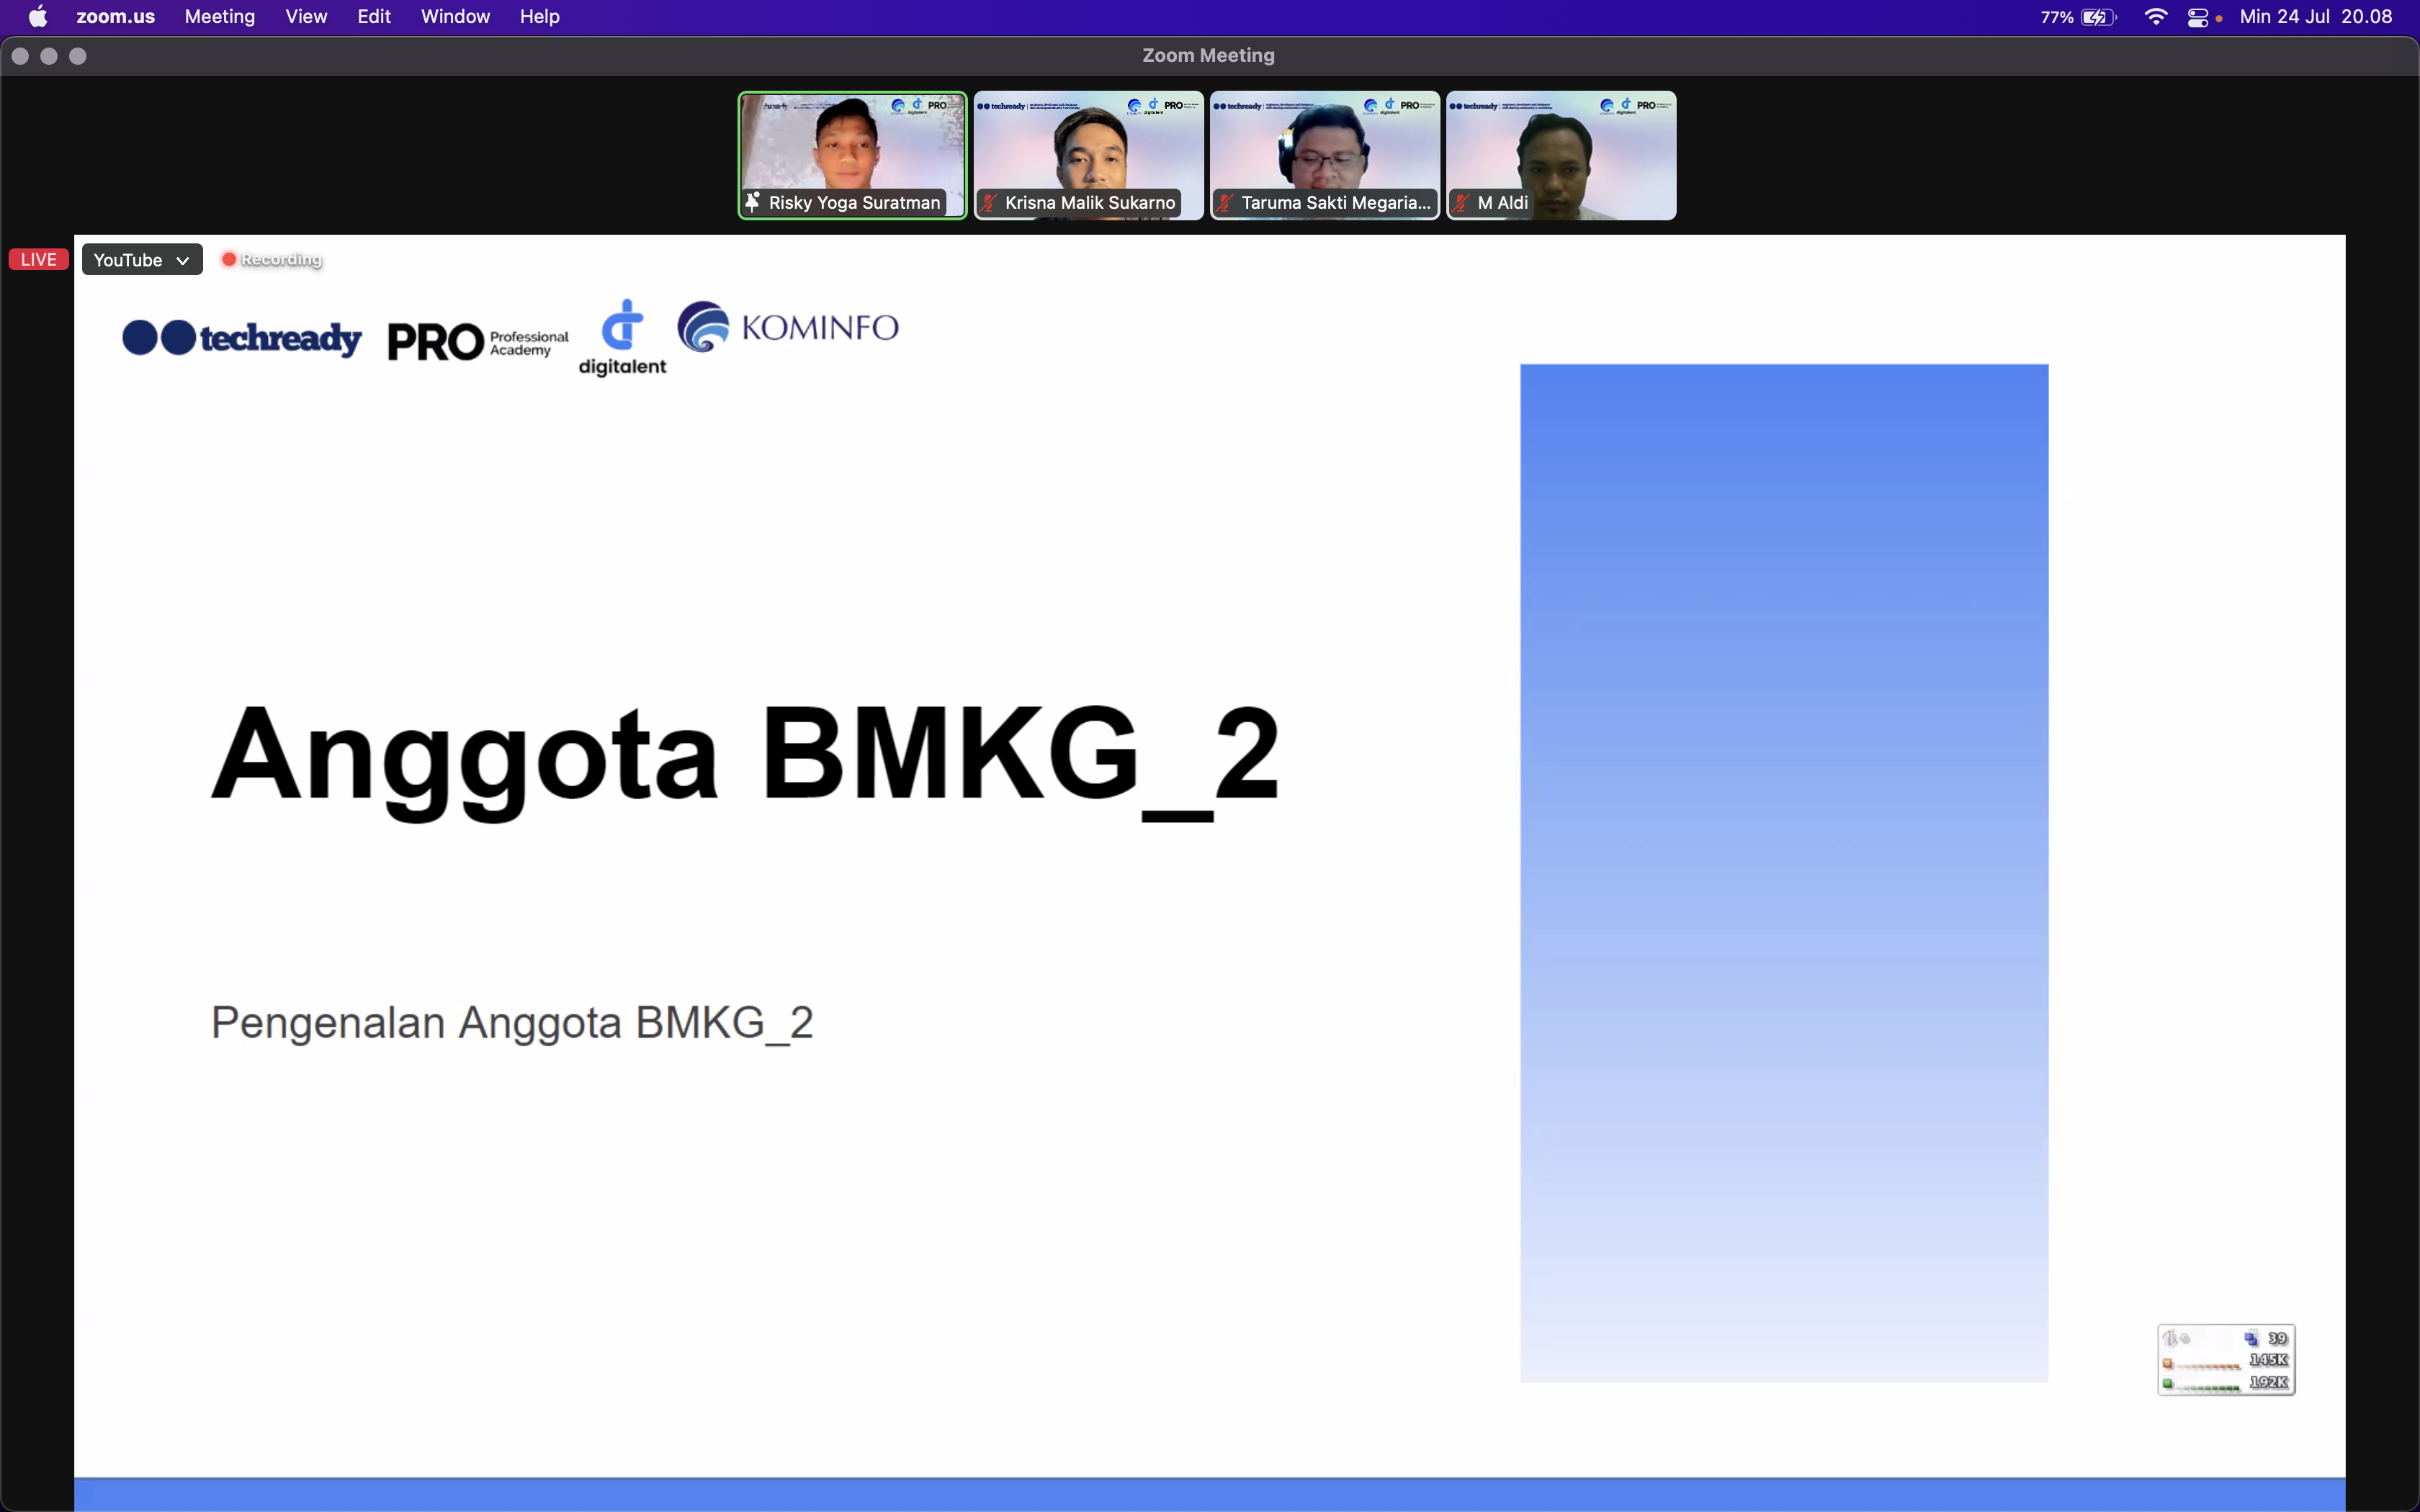
\includegraphics[width=\textwidth]{pert-4.3}
    \caption{Gladi Resik}
\end{figure}

\begin{figure}[h]
    \centering
    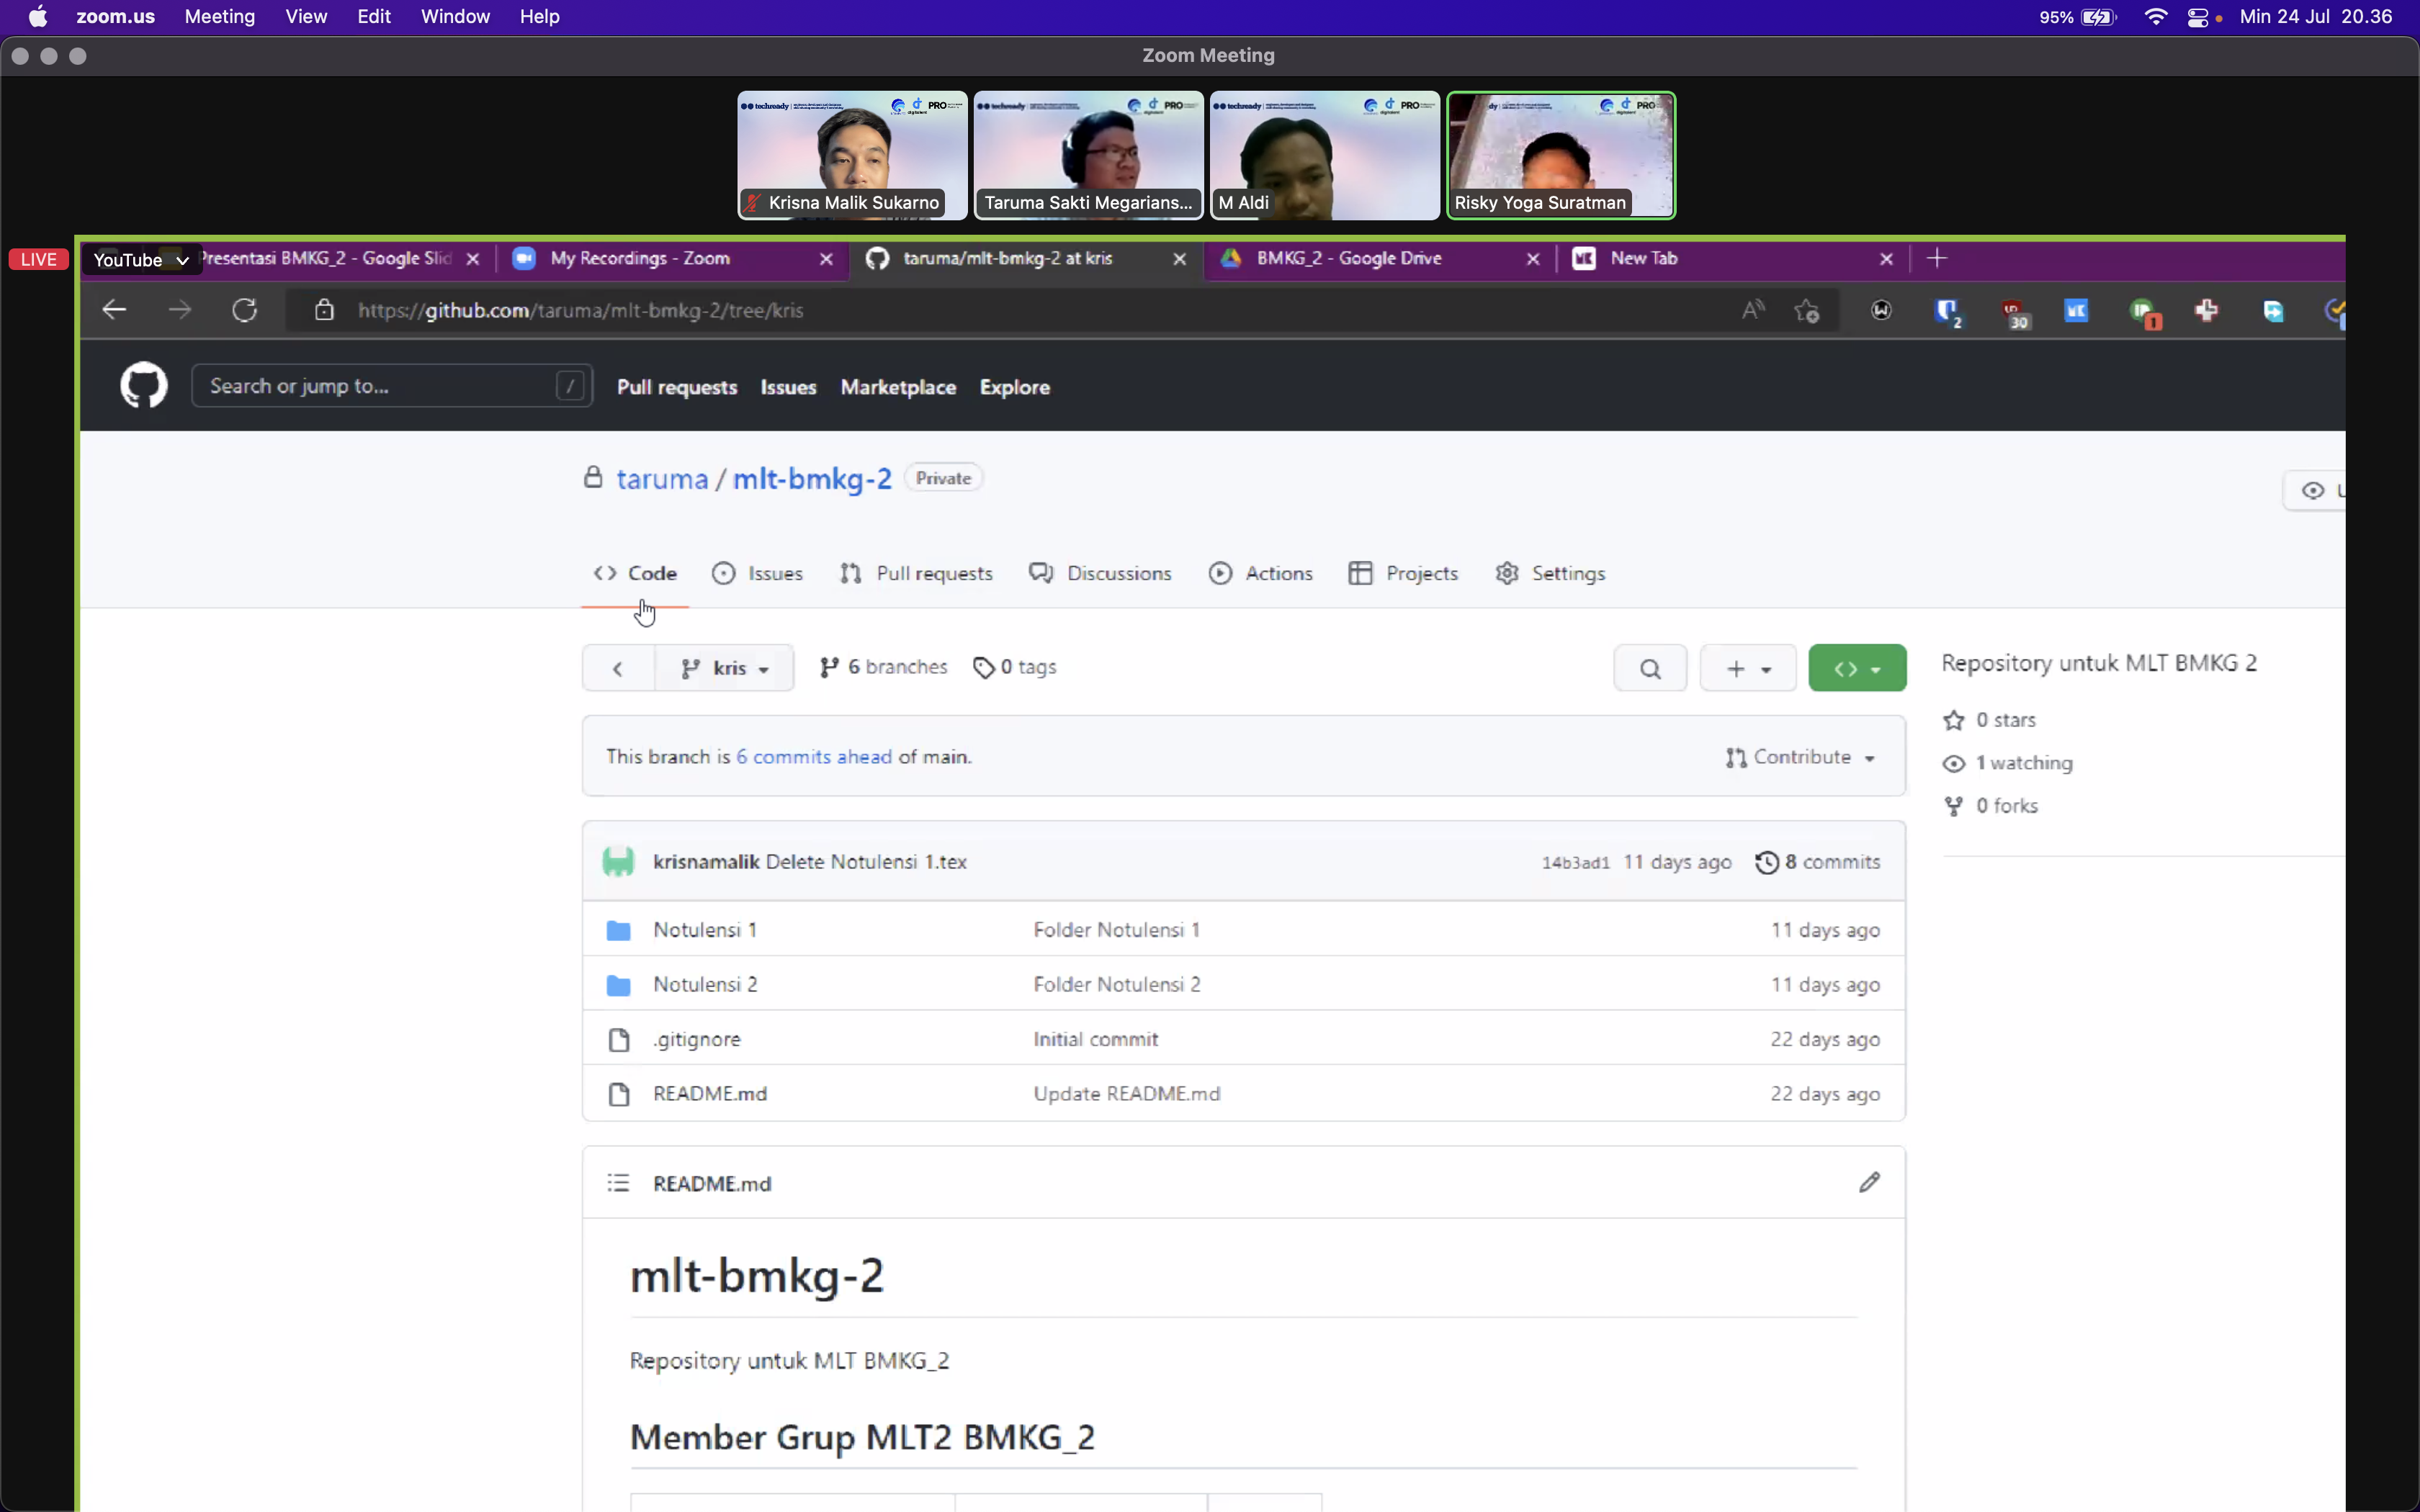
\includegraphics[width=\textwidth]{pert-4.4}
    \caption{Diskusi Terkait Github}
\end{figure}


\end{document}